\documentclass[main.tex]{subfiles}
\begin{document}
\glsresetall

\section{Introduction}

\glspl{iact} work detecting the Cherenkov light produced by the interaction of $\gamma$-rays and other particles in the
atmosphere. These Cherenkov photons must be distinguished from those of the \gls{nsb} that fill the atmosphere, and constantly reach the telescopes. An efficient trigger system is necessary to decide whether the light reaching the camera must be stored as a Cherenkov event, or discarded as background.
Typically this task is accomplished by recognizing a concentration of signal from several pixels both in space and time which would belong to a shower, while \gls{nsb} light is randomly distributed over the entire camera.\\
Two possible approaches for the detection of coincident light are used in \glspl{iact}, known as \textit{majority trigger} and \textit{sum trigger}. In majority trigger the light of each pixel is compared to a certain
threshold. If the signal of most pixels in a certain region exceeds the threshold in a short time, the trigger is fired. This approach presents a disadvantage when detecting low energy photon showers, as happens in \gls{lst}. The problem is that as the pixels must overcome the threshold individually, therefore, if the signal is too low, it is possible that not enough of them exceed the threshold and therefore the event would be interpreted as \gls{nsb}. On the other hand, the sum trigger approach takes into account the total signal coming to a group of several pixels. The light arriving at each pixel of the group is added and this sum is compared to a threshold to fire the trigger. If several close groups of pixels surpass the threshold at a given time window, then the event is recorded as a shower event.\\
In the LST, a multilevel trigger system is implemented, that guarantees the rejection of the majority of the \gls{nsb}.
The pixels in the \gls{lst} camera are distributed in 265 hexagonal modules of 7 pixels, that are connected to each of its 6 neighbors.
The first trigger level (L0) sums the signal of the pixels in each module, and if it is higher than the configured threshold, it sends the L0 signal to the neighboring modules. In the second trigger level (L1), each module takes the trigger signal coming from its neighbors and
compares it to another threshold to decide if the camera trigger is fired. Finally, the third level compares the camera trigger of
several telescopes and if two or more telescopes have triggered in a certain time window, the event is recorded. A scheme of the trigger system of \gls{lst} is shown in picture \ref{fig:trigger}. In the next sections, a detailed description of the three trigger levels is given.

\begin{figure}[h]
  \centering
  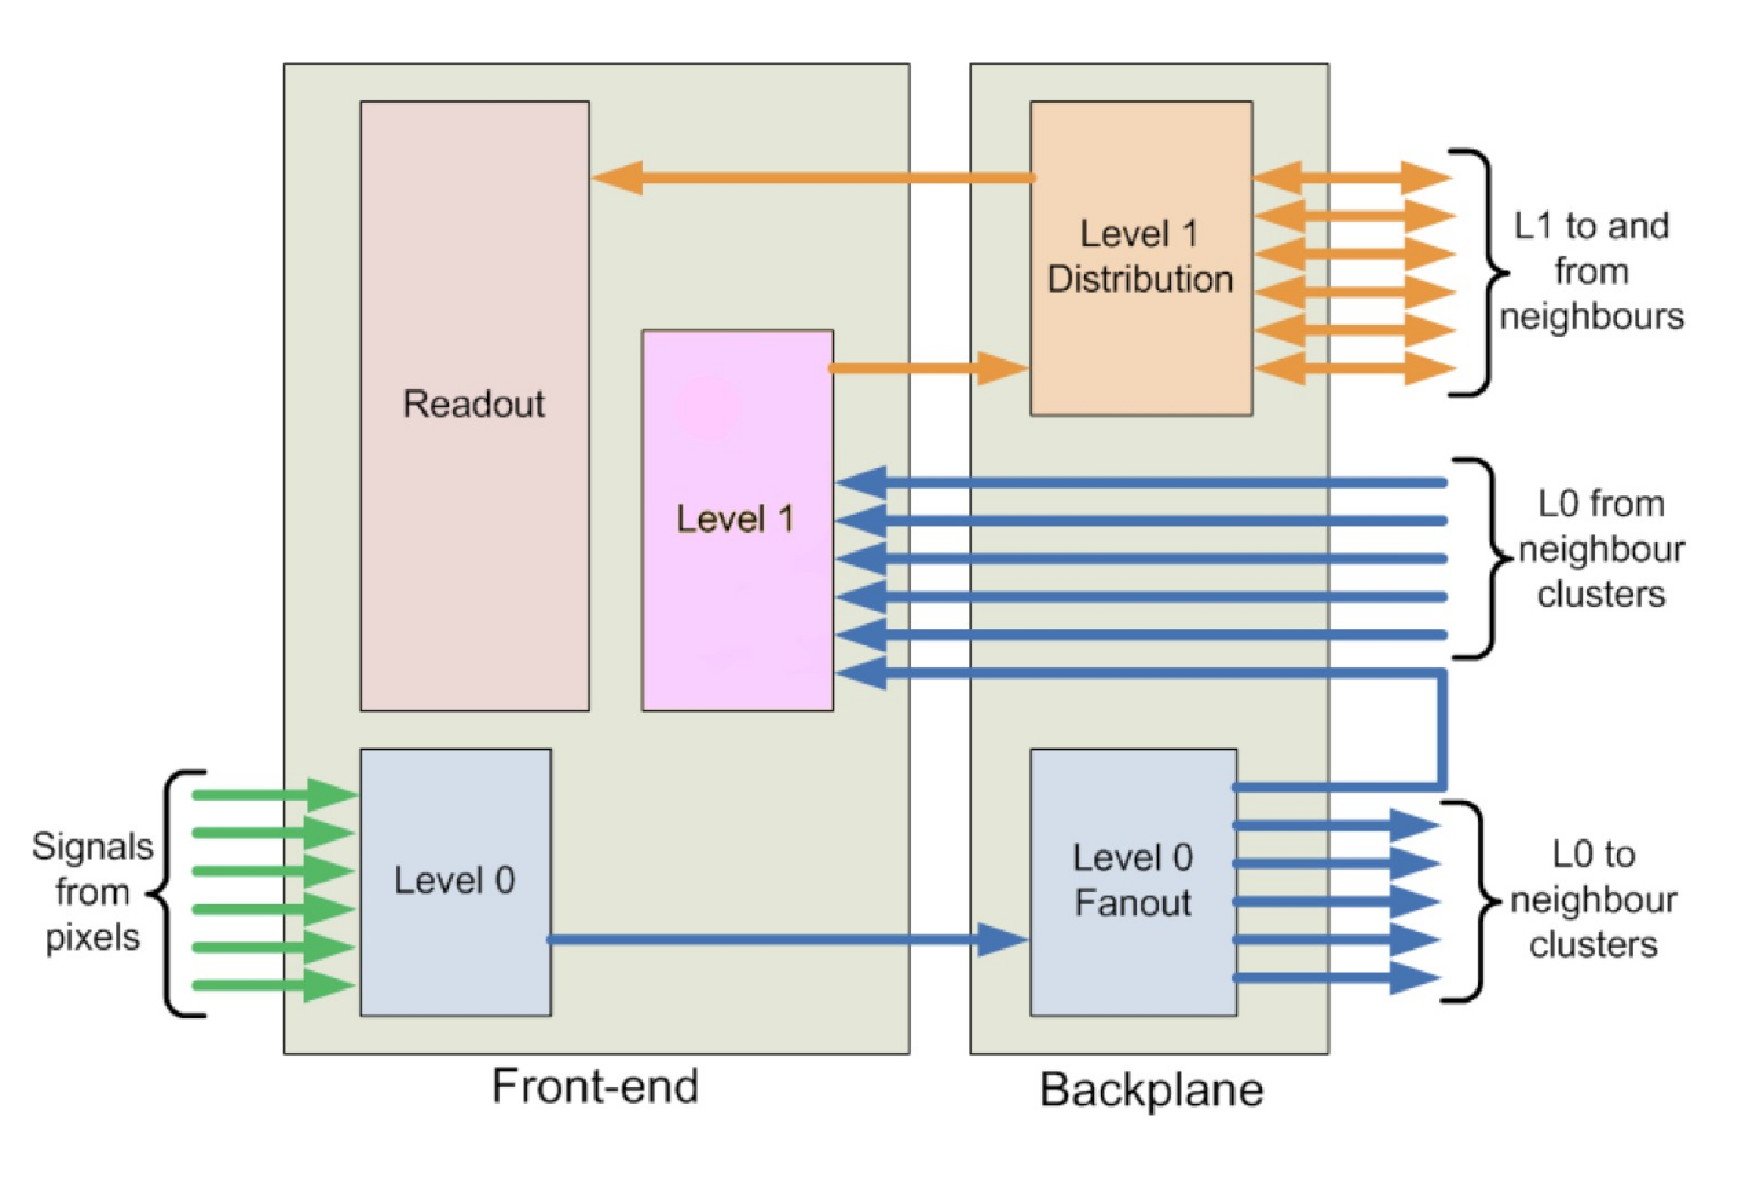
\includegraphics[width=0.7\textwidth]{./Pictures/triggerscheme.pdf}
  % L1blockdiagram.png: 1296x675 pixel, 72dpi, 45.72x23.81 cm, bb=0 0 1296 675
  \caption{Architecture of the analog trigger system of the \gls{lst}.}
  \label{fig:trigger}
\end{figure}


\section{Pixel Level: L0 trigger decision}

The pixel-level trigger, known as L0, takes into account the signals from the pixels in one module or cluster. If the trigger is fired, the signal is replicated and distributed by the L0 fan out to the local L1 and the neighboring modules. Both, the majority and sum trigger approaches have been implemented in \gls{lst}.

\subsection{Majority trigger}

The majority approach counts the number of pixels in a module that have a signal over a certain threshold voltage, generating a digital signal. The signal from all the pixels is added, with a resulting amplitude proportional to the number of activated pixels, that goes to the local L1 trigger system, and the neighboring modules. This approach does not account for the number of photoelectrons that activated each pixel, only for the number of pixels that have surpassed the threshold. This means that even if a large number of pixels in a region receive a flash of light but in each pixel the amount of photoelectrons is not over the threshold, the event will not be recorded, possibly losing very low energy events.

\subsection{Sum trigger}

The sum trigger adds the signal received in each pixel of the module and the resulting signal is compared with a threshold voltage. If
the threshold is surpassed, the signal is sent to local L1 and neighboring modules. This way makes it possible to take into account the photoelectron contribution of all pixels of the module, raising the sensitivity to low energy events while still rejecting \gls{nsb} events. After adding the signals of all pixels, a clipping is applied to overcome afterpulse effects in the photomultipliers. Afterpulses are sometimes produced after a real pulse in the photosensors, due to the ionization of residual gases, and can contribute with a very high amplitude to the sum.

\subsection{Camera Level: L1 trigger decision}

Camera level trigger decision system, known as  L1, analogically adds the resulting signals of L0 trigger from neighboring modules and compares
the result with a threshold voltage. If the analog sum is over the configured threshold, a signal is sent through the L1 distribution system to trigger the whole camera.
Each module can combine the L0 fan-out signals from six neighbors, plus the local L1. To ensure that all modules are participating in the trigger efficiently, it is possible to configure by slow-control different modes of adding configurations. In figure~\ref{fig:trigmodes} the three possible modes are shown. These configurations make it possible, through combinations of two, three, or four modules, to evaluate any trigger region.

\begin{figure}[h]
  \centering
  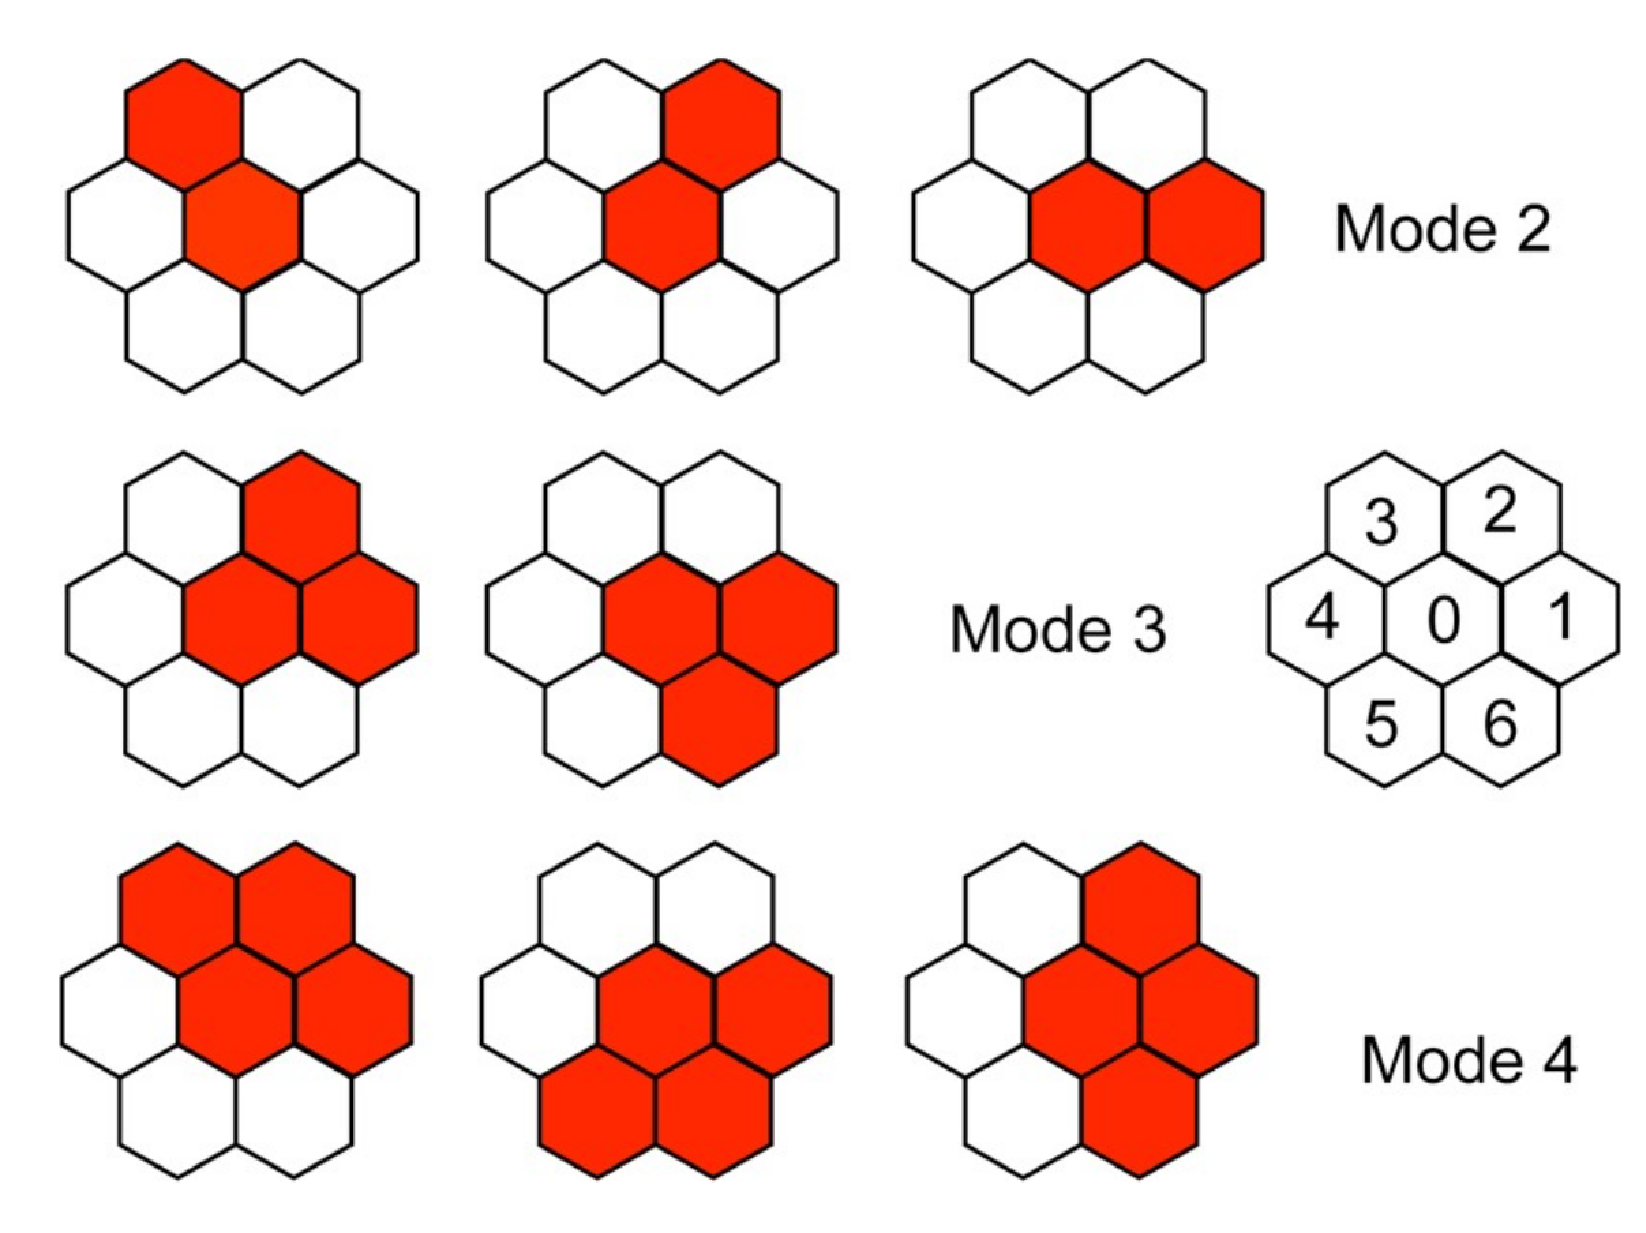
\includegraphics[width=0.5\textwidth]{./Pictures/triggermodes.pdf}
  \caption{Illustration of the three possible modes for adding signals of neighbouring modules. Each hexagon represents a group of seven photomultipliers.}
  \label{fig:trigmodes}
\end{figure}

The threshold voltages for each module should be calibrated to find the threshold level which produces a trigger signal at a rate of 50\%. The calibration algorithm developed for \gls{lst} camera is described in appendix \ref{app:calib}.

\subsubsection{L1 Trigger Distribution}

The L1 trigger distribution system allows the L1 signal to reach the data acquisition systems of all the modules and start the digitalizing process. Every module can propagate the L1 signal to each of its six neighbors, being aware of its position in the camera. This way, when a module receives an L1 signal, it can be delayed depending on its position in the camera, and be sent to the appropriate neighbors following the preconfigured paths (See figure ~\ref{fig:trigpaths}). The distribution paths are firmware configurable and they can automatically be reconfigured to go through the full camera, even if one module is malfunctioning or deactivated. The algorithm developed for the time delay calibration of the L1 signal is described in appendix \ref{app:timecal}.

\begin{figure}[h]
  \centering
  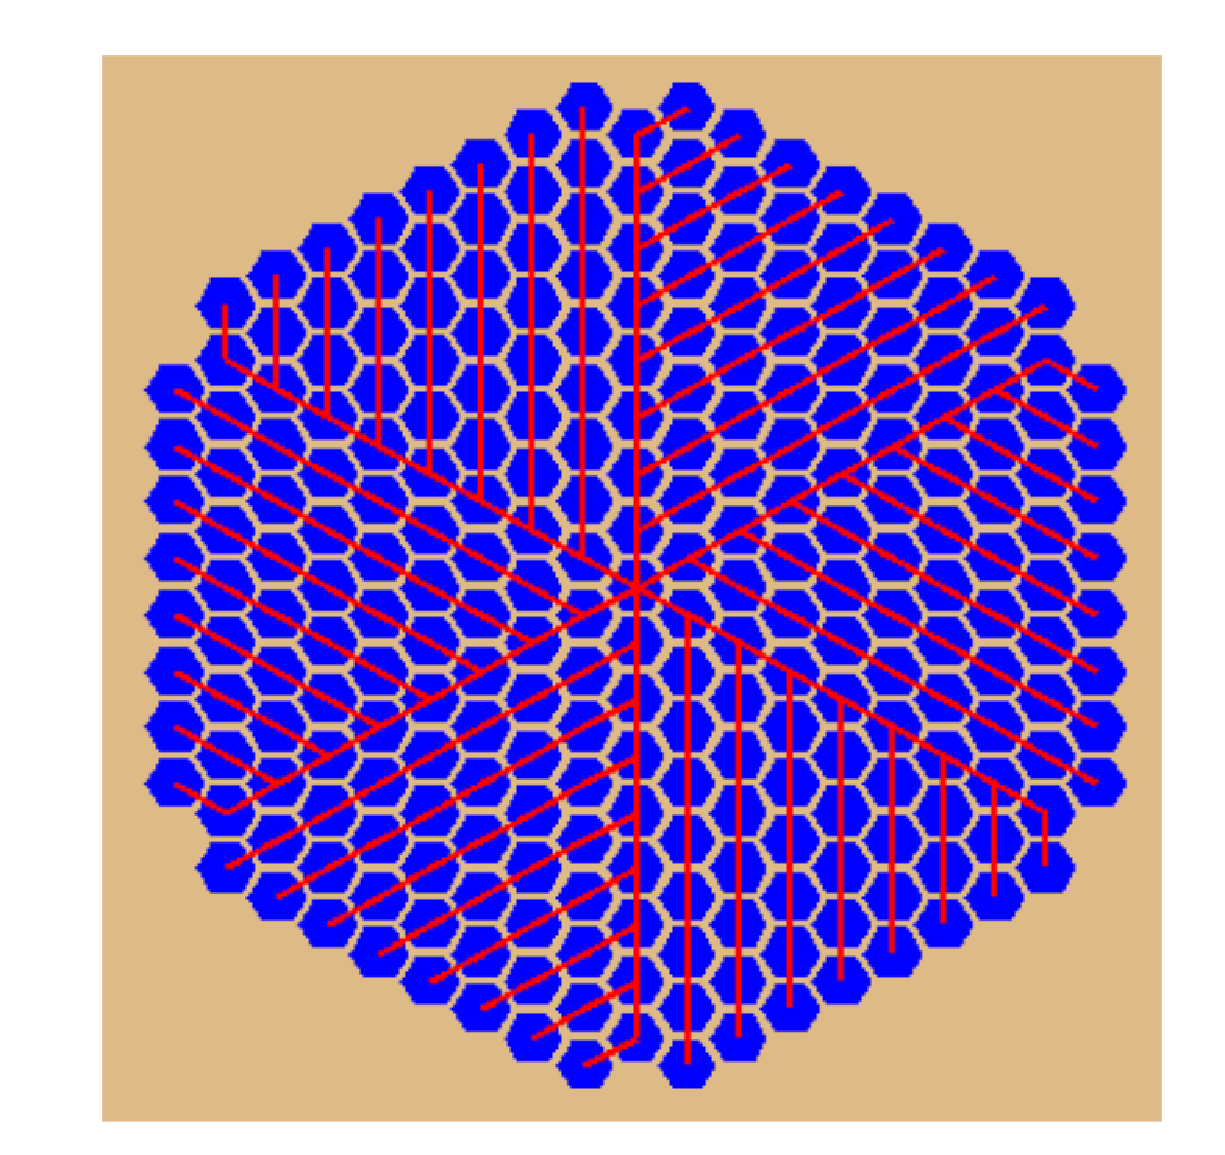
\includegraphics[width=0.7\textwidth]{./Pictures/triggerpaths.pdf}
  % L1blockdiagram.png: 1296x675 pixel, 72dpi, 45.72x23.81 cm, bb=0 0 1296 675
  \caption{Paths for trigger distribution over the entire camera.}
  \label{fig:trigpaths}
\end{figure}

\subsection{Array Level trigger decision}

Array level trigger looks for coincidences in events recorded by several telescopes. If more than one telescope produces a camera trigger in a certain time window, the light is likely produced by a Cherenkov shower, so the event will be stored. This level rejects the majority of \gls{nsb} events that have overcome the lower level triggers.

\end{document}
